\question{Спонтанные и индуцированные переходы. Коэффициенты Эйнштейна}

\subquestion{Спонтанные и индуцированные переходы}

\emph{Спонтанные переходы} -- самопроизвольные переходы квантовой систем
из состояния с высокой энергией в состояние с низкой энергией.

\emph{Индуцированные (вынужденные) переходы} -- переходы между уровнями энергии
квантовой системы под действием внешнего излучения, энергия квантов которого
равна разнице уровней. В отличие от спонтанных, происходят как сверху вниз, так
и снизу вверх и зависят от интенсивности внешнего излучения.

\subquestion{Коэффициенты Эйнштейна}

\begin{figure}[h!]
    \center
    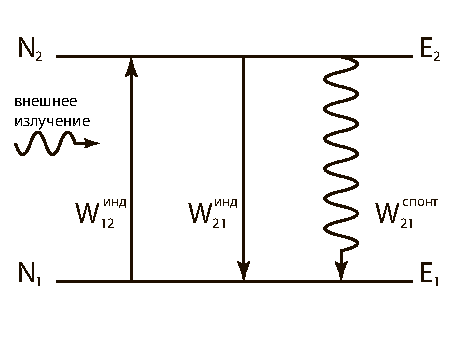
\includegraphics[width=.4\textwidth]{06_01}
\end{figure}
Здесь
\begin{itemize}
    \item \( W_{21}^\text{сп} = A_{21} \) -- вероятность самопроизвольного
        перехода в единицу времени;
    \item \( W_{21}^\text{ин} = B_{21}\rho_\nu \) -- вероятность индуцированного
        излучения в единицу времени;
    \item \( W_{12}^\text{ин} = B_{12}\rho_\nu \) -- вероятность индуцированного
        поглощения в единицу времени;
\end{itemize}

\( A_{21} \) -- это вероятность самопроизвольного перехода из состояния
\( 2 \) в состояние \( 1 \) в единицу времени. Её называют коэффициентом
Эйнштейна для спонтанных переходов.

\( B_{12} \), \( B_{21} \) -- вероятность вынужденного перехода
\( 1 \rightarrow 2 \) (\( 2 \rightarrow 1 \)) в единицу времени, отнесённая к
спектральной объёмной плотности излучения \( \rho_\nu \). Их называют
коэффициентами Эйнштейна для индуцированного поглощения и излучения
соответственно.

